%
\documentclass[12pt]{report}
\usepackage{setspace}
%\usepackage{subfigure}

\pagestyle{plain}
\usepackage{amssymb,graphicx,color}
\usepackage{amsfonts}
\usepackage{latexsym}
\usepackage{a4wide}
\usepackage{amsmath}
\usepackage{diagbox}

\graphicspath{{figures/}}

\usepackage{hyperref}
\usepackage[all]{hypcap}
\usepackage{float}

\usepackage[utf8]{inputenc}
\usepackage[english]{babel}
\usepackage[nottoc]{tocbibind}
\allowdisplaybreaks

\newtheorem{theorem}{THEOREM}
\newtheorem{lemma}[theorem]{LEMMA}
\newtheorem{corollary}[theorem]{COROLLARY}
\newtheorem{proposition}[theorem]{PROPOSITION}
\newtheorem{remark}[theorem]{REMARK}
\newtheorem{definition}[theorem]{DEFINITION}
\newtheorem{fact}[theorem]{FACT}

\newtheorem{problem}[theorem]{PROBLEM}
\newtheorem{exercise}[theorem]{EXERCISE}
\def \set#1{\{#1\} }

\newenvironment{proof}{
PROOF:
\begin{quotation}}{
$\Box$ \end{quotation}}

\newcommand{\nats}{\mbox{\( \mathbb N \)}}
\newcommand{\rat}{\mbox{\(\mathbb Q\)}}
\newcommand{\rats}{\mbox{\(\mathbb Q\)}}
\newcommand{\reals}{\mbox{\(\mathbb R\)}}
\newcommand{\ints}{\mbox{\(\mathbb Z\)}}

%%%%%%%%%%%%%%%%%%%%%%%%%%


\title{         { 
\includegraphics[scale=.5]{ucl_logo.png}}\\
{{\Huge \textbf{Multi-hop Question Answering with\\ Link Completed Graph}}}\\
% {\large Optional Subtitle}\\
                }
\date{September 2019}
\author{Yangguang Li\thanks{
{\bf Disclaimer:}
This report is submitted as part requirement for the MSc degree in Computational Statistics and Machine Learning at University College London. It is
substantially the result of my own work except where explicitly indicated in the text. The report may
be freely copied and distributed provided the source is explicitly acknowledged.}
\\ \\
MSc Computational Statistics and Machine Learning\\ \\
Supervisor: Prof. Philip Treleaven\\
Industrial Supervisor: Marcelo Gutierrez}



\begin{document}

 \onehalfspacing
\maketitle
\begin{abstract}
\begin{singlespace}
Question answering (QA) requires the system to answer a given question by: choosing a candidate among a given list, extract the answer from given text, or recall from the system's own knowledge bases. Also the question may come with supporting text, images, or videos. Previously researcher were focusing on answering questions with only one single supporting text, while in the real world people usually find the answer for a particular question by looking through and combining information from several sources. Hence recently more researchers are putting efforts into tacking multi-hop QA (MHQA): questions that can only be answered by combining factoid information from multiple sources. Among them, some researchers have successfully used relational graph and contextual embedder to achieve state-of-the-art (SOTA) result.

This dissertation investigates the possibility of utilizing link prediction on graphs as an auxiliary
task of multi-hop question answering problem, i.e. to improve MHQA by completing the graphs used
for inference. This is important because graphs are known to be incomplete, and filling in those missing information by link prediction may help capturing the reasoning chains in the propagation steps in graphs.
Though people have achieved near human-level performance in single-document QA, most of the architectures designed for that setting fall behind in the multi-document setting. Some researches have started to tackle this problem, but they are still far from achieving human-level performance, not to mention solving it. One of the reason that stops graph-based methods to get better performance maybe the missing of information in the graphs.

This research comprises:
\begin{enumerate}
\item Extract the named entities and coreference chains from the query and its supporting documents to form the nodes and edges of the relational graph;
\item Encode the mentions of candidates and query contextually to get the initial embedding of nodes with Embeddings from Language Models (ELMo) \cite{peters_deep_2018};
\item Propagate the information hold in the graph along the edges with Relational Graph Convolutional Network (R-GCN) \cite{schlichtkrull_modeling_2018};
\item Use an output layer to choose the node with highest probability as the answer.
\item Perform link prediction before propagate the information and test whether the link prediction has improved the MHQA performance.
\end{enumerate}

The models are built with PyTorch and PyTorch Geometric (PyG) and run on Graphics processing unit (GPU). Implementing them this way significantly shortens the running time comparing to the papers which did the experiments on Central processing unit (CPU) \cite{schlichtkrull_modeling_2018, de_cao_question_2019}. Some of the graphs are too large to put in the memory of GPU. In order to process them, mix precision training is used \cite{micikevicius_mixed_2017}.

The testing is done with the QAngaroo \cite{welbl_constructing_2018} dataset, particularly its unmasked WikiHop dataset. The dataset contains 43738 training instances and 5129 development instances. As the testing set is not published, the evaluation is done on the development set only, i.e. the development set is blinded.

[\textbf{TODO} Result]

\end{singlespace}
\end{abstract}

\tableofcontents

% \setcounter{page}{1}
\listoffigures
\listoftables


\chapter{Introduction}
This chapter presents an overview of the dissertation. It starts with introducing the research topic and state the motivation of this project. Then the objective of this project is further explained, which is followed by the discussion of the dataset used and the structure of this dissertation.

\section{Problem and Motivation}
Question answering is about building a system that can read in textual corpus, reason on it, and achieve a conclusion. It is a longstanding goal in the fields of information retrieval and natural language processing (NLP). With such a system, we will be able to input text files, audio, and/or videos to the system, and get the answer to questions concerning those files that have not being processed manually.

A typical way to assess such a system is by evaluating its performance on question answering datasets. Such
a dataset is specifically prepared as a set of questions $\{A\}$, where each question $A$ consists of
a query $q$ and the correct answer $\bar{c}$. Sometimes there may also be supporting document(s) $\{d\}$
and a list of candidates $\{c\}$ being provided. The system is required to answer the query based on
the supporting document(s) or some common knowledge/knowledge bases it has in itself. If the candidates
is provided, the system just need to pick one of them; otherwise it needs to extract the correct answer
of free-form text from the whole span of the given text.

Previous researches mainly focused on QA based on only a single document or paragraph. Boosted by the
availability of large-scale datasets like SQuAD \cite{rajpurkar_squad:_2016} and CNN/Daily Mail \cite{hermann_teaching_2015}
in which most questions can be answered by attending the information in only one single sentence,
 many end-to-end neural models \cite{seo_bidirectional_2016, xiong_dynamic_2016, shen_reasonet:_2017}
have been proposed and achieved good performances on these datasets. To overcome the limit of these datasets
\cite{weissenborn_making_2017}: requiring only the information from one single sentence to answer the
questions, people have proposed NarrativeQA \cite{kocisky_narrativeqa_2018}, CoQA \cite{reddy_coqa:_2019},
TriviaQA \cite{joshi_triviaqa:_2017}, and RACE \cite{lai_race:_2017} which have questions that can only
be answered if information from multiple sentences within the same document is gathered together.
Though being more challenging, the several sentences for each document are still strongly related as there are usually some kind of logical flows among the sentences in the same document.

In the real word, when given a question, people usually go to sources of different topics, written by people of various backgrounds and for audiences of diverse interests. Hence the capability to combine sources that are so heterogenous is desired for QA systems. With such a system, we are able to input unstructured data that remain unprocessed to the system and ask arbitrary questions of interest. Attracted by this topic, a dataset named QAngaroo \cite{welbl_constructing_2018}, which will be discussed in more details later, is constructed specifically for tackling multi-document QA problems. Researcher started from simply
concatenating the documents into a big one, and then applied the architectures, namely attention-based methods \cite{seo_bidirectional_2016, weissenborn_making_2017}, developed for single-document QA.
The results were presentable but far from human-level performance, the level those attention-based models have achieved in single-document QA datasets.

Another branch of research on this topic utilized the graph extracted from the query and its supporting documents \cite{de_cao_question_2019, song_exploring_2018, tu_multi-hop_2019}. They then propagated the information along the edges  extracted with Graph Neural Network (GNN) \cite{zhou_graph_2018} namely Graph Convolutional Network \cite{kipf_semi-supervised_2016}, Graph Recurrent Network \cite{li_gated_2015, zhang_sentence-state_2018, song_graph--sequence_2018}, and Graph Attention Network\cite{velickovic_graph_2017}. People believed that the reasoning chain could be captured by the propagation steps. This kind of approaches have improved the performance on QAngaroo WikiHop and remain the SOTA.

However, the performances achieved by these graph-based methods are still far from human-level. I am hypothesising that the deficiency is caused by the missing of information from the constructed graph, as the way how the graphs were constructed are quite limiting: the nodes are exact match of candidates and query entity in the supporting documents, and the edges are just four kinds predefined relationships between those named entities.
\section{Objective}
The research objective is to improve the MHQA performance on QAngaroo WikiHop dataset by introducing link prediction into graph-based method, given the hypothesis that this method is limited by the missing of information from the constructed graphs.
To verify my hypothesis, I have implemented \cite{de_cao_question_2019} on GPU and compared
the results of the method with/without link prediction between graph construction and information propagation.


\section{Dataset}

Although remaining challenging, \cite{kocisky_narrativeqa_2018, reddy_coqa:_2019, joshi_triviaqa:_2017, lai_race:_2017} are created for reasoning within the same document, which
is not the case for many real-world applications that requires aggregating information from multiple
documents, or even from multimodal sources. In this dissertation we only focus on text question answering,
hence only tackling the case of multi-document QA. Seeing the need for a dataset to facilitate research
in MHQA, Welbl et al. released a new dataset named QAngaroo \cite{welbl_constructing_2018} which consists
of WikiHop and MedHop.

The dataset requires the system to reason across multiple supporting documents
before it can achieve the conclusion to pick the right answer among the candidates. WikiHop consists
of questions generated from the user-created multi-domain unstructured text corpus Wikipedia and the
structured information set Wikidata. All the information needed for answering a particular query is contained
in the supporting documents, but there may also be some misleading documents which penalise the systems
that perform only exact matches without comprehending the context in the reasoning procedure.

In Figure
\ref{wikihop_example}, we show an example of WikiHop dataset where the system need to combine information
from several documents to get the correct answer to the question. We can see the appearance of misleading
document in the example: in the first document we get \textit{Mumbai} being adjacent to the \textit{Arabian
Sea}, and in the last document we find that \textit{Arabian Sea} is closer to \textit{Pakistan} and \textit{Iran}
than the correct answer, \textit{India}, does in terms of the relational positions in the text. In such
a scenario, a system that does not have semantic understanding of the context may fall into the trap
and pick \textit{Iran} or \textit{Pakistan} as the answer.

The MedHop dataset in QAngaroo is about finding
the drug that will interact with a given drug according the provided text from PubMed, a dataset of biomedical
literatures. The supporting documents are abstracts of research papers, and al candidates are drugs'
names extracted from the whole text corpus. This dataset is much smaller comparing to WikiHop: 2,508
instances versus the 51,318 ones of the WikiHop. Also the text are closed-domain now, hence the requirement
on the ability to do reading comprehension is lower than that of WikiHop.
Therefore we are only focusing on WikiHop instead of MedHop.
\begin{figure}[H]
\centering
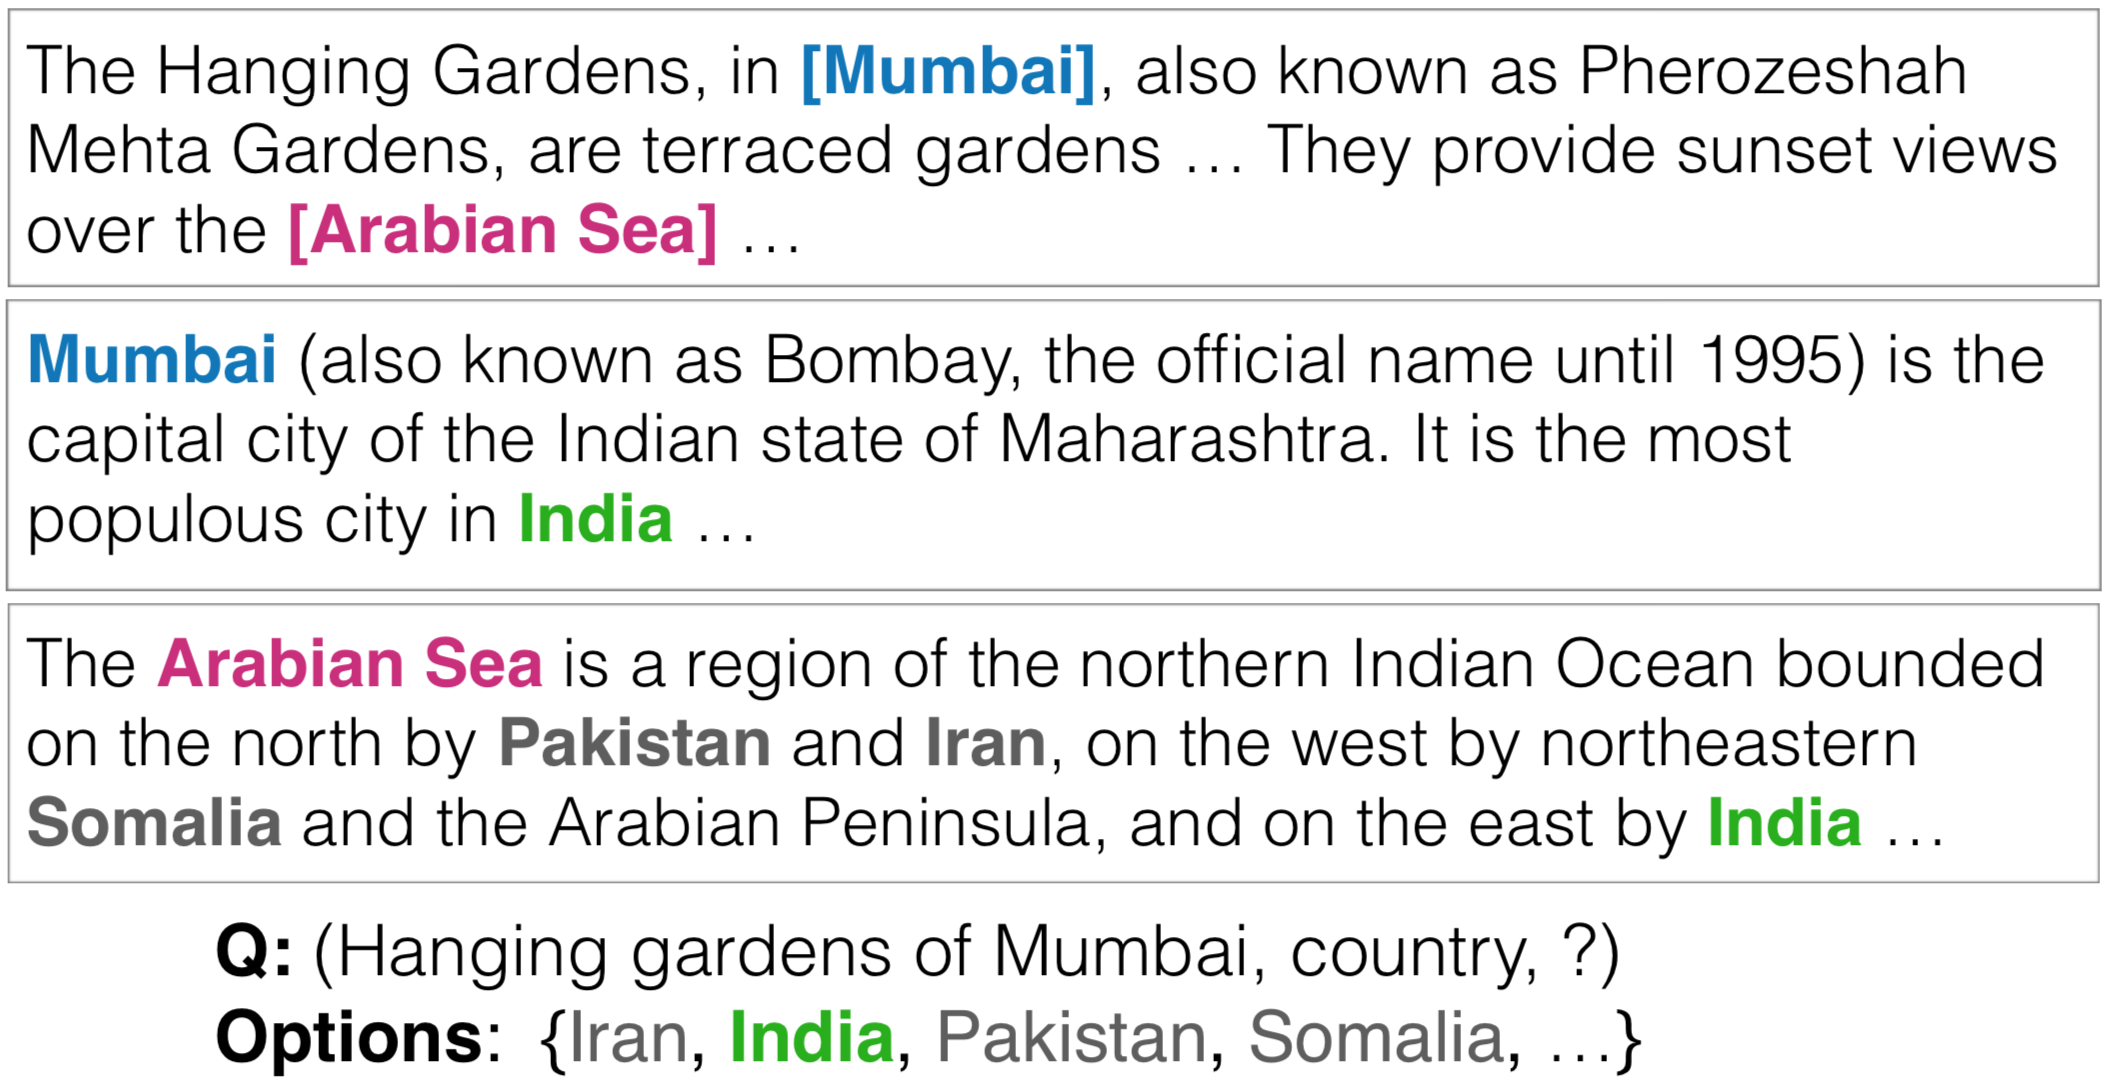
\includegraphics[width=0.9\textwidth]{figures/wikihop_example.png}
\label{wikihop_example}
\caption[An example from the WikiHop dataset]{An example from the WikiHop dataset. Reprinted from \cite{welbl_constructing_2018}.}
\end{figure}

\section{Structure of the Dissertation}
Structure of this dissertation is as follows,
\begin{itemize}
\item Chapter 2 reviews the background in a number of key areas including NLP, GNNs, and link prediction. Then the related work is briefly describes.
\item Chapter 3
\item Chapter 4
\item Chapter 5
\end{itemize}


\chapter{Background and Related Work}
This chapter starts with introducing the background knowledge needed to understand the related work. Then it goes to briefly describes the literature related to my work.

\section{Background}
This section includes key concepts needed in NLP, GNNs, and link prediction.

\subsection{Natural Language Processing}
NLP is a subfield of computer science concerned with processing and analyzing large amount of natural language data. Inspiring by the famous paper of Alan Turing \cite{turing_i.computing_1950} on Turing test, researchers have put much efforts into solving NLP problems relating to:
\begin{itemize}
\item Syntax: part-of-speech tagging, lemmatization, and parsing;
\item Semantics: machine translation, named-entity recognition (NER) \cite{strubell_fast_2017}, natural language understanding, QA \cite{andrenucci_automated_2005}, and textual entailment;
\item Discourse: coreference resolution \cite{wiseman_learning_2016, clark_deep_2016, martschat_latent_2015}.
\end{itemize}

In the early days, many NLP systems were constructed with hand-crafted rules, which imposed a consequential limit on their abilities: the systems were not able to handle the variations that had not been encoded into the system by human. In order to equip those systems with the capacity for solving cases they have not encountered, researchers introduced machine learning (ML), a field that studies how to automate computer programs,
into the systems.
\subsubsection{Neural Network} ML studies how to find patterns in data efficiently and exploit the finding to perform a specific task automatically \cite{bishop_pattern_2006}. Assuming a mathematical model over the data, ML algorithms learn the parameters and infer the latent variables from the data \cite{barber_bayesian_2012}. Ranging from linear regression \cite{freedman_statistical_2009} to Gaussian process \cite{rasmussen_gaussian_2004}, there are various families of ML models available for solving different problems. In the field of NLP, one of the most important kind of data is unstructured data which is text-heavy. In order to process them we usually treat those data as sequential data and use Markov models such as n-gram model \cite{jurafsky_speech_2000} which assumes that the next word/letter statistically depends only on the past n words:
\[p(x_i|x_{i-(n-1)},\dots,x_{i-1})\]
This assumption considerably simplified the search space of the language model, and led to many successful applications.

More recently, Recurrent Neural Network (RNN) \cite{elman_finding_1990}, an extension of standard multi-layer perceptron \cite{van_der_malsburg_frank_1986}, had been proposed to
deal with sequential data and time-series data. The network maintains a hidden state that can change over steps, and takes in input, like tokens or price of stock, one at a time. Then it apply a learned transformation to the concatenation of input and hidden state to produce the output and hidden state for the next step:
\begin{align*}
h_{t} &= \sigma(W^xx_t+W^hh_{t-1}+b)\\
&= \sigma(W[x_t;h_{t-1}]+b),\\
o_{t} &= \tau(h_{t}),
\end{align*}
where $h_t, h_{t-1}$ are hidden states at the end of steps $t$ and $t-1$, $x_t$ is the input at step $t$, $W, b$ are weights to learn, and $\sigma$, usually $tanh$ or $relu$, is the non-linearity applied. Usually chosen as identity mapping, $\tau$ is the function that maps hidden state to output. As a general function approximator, RNN is more powerful then n-gram models and can theoretically process sequences, i.e. sentences, of arbitrary size.

However, at the time when RNN was proposed, people were suffering from the inefficiency of computing power that was needed to train the network with Backpropagation Through Time (BPTT). Even if computing BPTT was feasible, they still faced the problem of gradient exploding and gradient vanishing. To solve these problems, Hochreiter and Schmidhuber proposed Long Short-Term Memory (LSTM) network which introduced gating mechanism to control how much the hidden state, i.e. the memory, is updated given the input:
\begin{align*}
h_{t-1}, c_{t-1} &= s_{t-1},\\
z_t &= [x_t; h_{t-1}],\\
i_t &= \sigma(W^iz_t+b^i), \text{ input gate}\\
f_t &= \sigma(W^fz_t+b^f), \text{ forget gate}\\
o_t &= \sigma(W^oz_t+b^o), \text{ output gate}\\
c_t &= f_t \odot c_{t-1} + i_t \odot tanh(W^cz_t+b^c),\\
h_t &= o_t \odot tanh(c_t),\\
s_t &= [h_t; c_t],
\end{align*}
where $h_t$ and $c_t$ is the hidden state and cell state at step $t$, $x_t$ is the input at step $t$, $\sigma$ is the sigmoid function, and all $W^\cdot, b^\cdot$s are the weight to be learned.

Given the chance that the LSTM can retain some of the memory instead of updating it completely as did in vanilla RNN, it introduces a `short-cut' for the backpropagation of gradient, and gets rid of the exploding/vanishing gradient caused by the weight matrix having its largest eigenvalue being not equal to one. In this dissertation I have used Bidirectional LSTM (BiLSTM) to encode the query. Proposed by Graves et al. in 2013 \cite{graves_speech_2013}, this model adds a pipeline that process the sequence in the reversed order as shown in Figure \ref{bilstm}, hence it can combine not only the information from the past but also from the future for each token. Empirically this bidirectional mechanism usually provides a better result than its unidirectional counterpart.
\begin{figure}[H]
\centering
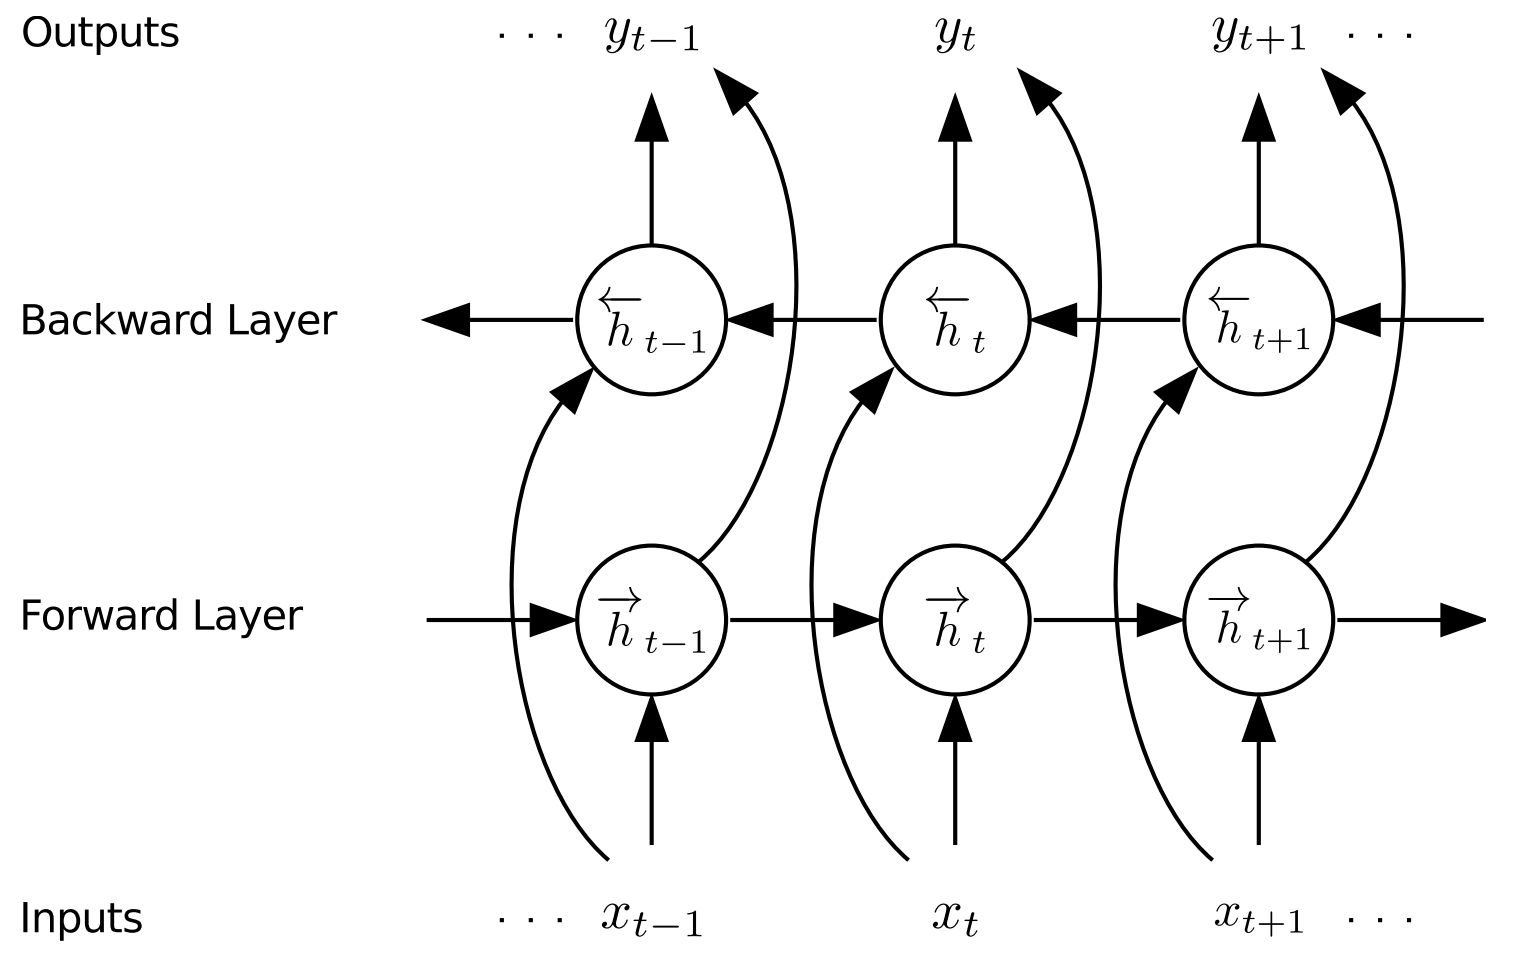
\includegraphics[width=0.45\textwidth]{figures/bilstm.png}
\label{bilstm}
\caption[BiLSTM]{BiLSTM. Reprinted from \cite{graves_speech_2013}.}
\end{figure}

\subsubsection{Loss}
For most ML algorithms, we train the model by either maximising the likelihood or posterior or minimising an expected loss. In this work the final metric is the accuracy of the model on the development set of WikiHop, and the way how the model makes prediction for each instance is by choosing the node with the highest probability. Hence it seems like we can regard this problem as a classification problem, where we naturally go to cross entropy (CE) loss:
\[loss(x, class) = -\log\left(\frac{\exp(x[class])}{\sum_j \exp(x[j])}\right) = -x[class] + \log\left(\sum_j \exp(x[j])\right), \]
where $x$ is a vector of logits produced by the output layer for each class i.e. each node in our problem, and $class$ the index of the correct node.

However, for one instance there maybe more than one correct node, which indicates the answer has appeared in supporting documents for more than once. It is then hard to define the target vector. For CE loss there should be only one correct class, hence for the target vector there is only one non-zero value on the position corresponding to the correct class. But there would be multiple non-zero values in the target vector in our problem, and if treated equally, they will be $1/n$ given there are $n$ nodes corresponding to the answer. This way we are having a target that is changing its amplitude across instances, and being inconsistent with the definition of CE loss.

Therefore I have used another loss function that is more suitable for this problem which may have multiple correct answers: Binary Cross Entropy (BCE) loss. The loss function can be written as:
\[loss(x, y) = \square_{i=1}^n [y_nlog(x_n)+(1-y_n)log(1-x_n)],\]
where $x$ is the logits aforementioned, $y$ is the target, $n$ is the number of nodes, and $\square$ is the reduction function which can be mean or sum. This way the target can be constructed as a vector of 0s and 1s where the non-zero values are on the positions corresponding to the correct nodes. Now the problem has transformed into a number of subproblems: whether a particular node is the correct answer or not.

\subsubsection{Optimisation}
People use optimisation methods to find the optimal or near-optimal solutions for problems. The problems in machine learning can be generalised as: given the hypothesised model over the dataset, what are the parameters that make the model optimally `fits' the data. In order to find those parameters, researchers have developed various methods that can be categorised into three main kinds: zero-order methods, first-order methods, and second-order methods.

Zero-order methods, like Particle Swarm Optimisation \cite{kennedy_particle_1995} and Evolutionary Algorithms \cite{angeline_evolutionary_1998}, utilise neither the gradient nor the Hessian information. Hence they are quite general but may suffer from slow running. The most common optimisation methods for models involving neural networks are first-order methods which use the gradient information to assist the searching for better parameters iteratively.
The last kind of methods that exploit both gradient and Hessian information is called second-order
methods. The Hessian information may help even more, but the approximation is only trustworthy in a local region and may underestimate curvatures along some directions.

Among first-order methods, Stochastic gradient descent (SGD) \cite{robbins_stochastic_1951} is the most popular optimisation method being used. It randomly samples a mini-batch from the whole dataset and use the gradient computed on that small batch to approximate the gradient. Therefore it generalise pretty well, and may be able to get rid of some of the local minimums. But
one of the drawbacks of SGD is that it uses fixed learning rate for all steps, which easily make the learning rate too big in the earlier stage and too small in the later stage. Moreover, the update variance of SGD is high because of lack of momentum. It also converges slowly if local curvature is too small, where momentum may assist in convergence.

Another first-order optimisation method, Adaptive Moment Estimation (Adam) \cite{kingma_adam:_2014}, is also commonly used. However, in spite of having faster convergence and lower variance, adaptive optimisation methods, such as Adam, has been found to generalize poorly comparing to SGD. These methods tend to perform well in the initial portion of the training but are outperformed by SGD at later stage of training \cite{wilson_marginal_2017}. Since the batch size is very small in my work due to the limit of GPU memory, Adam was used to stabilise the training procedural.

\subsubsection{Word Embedding}
A technique in NLP where words are mapped to numerical vectors, word embedding has boosted the performance in many downstream tasks such as semantic analysis and machine translation. The relative locations of the vectors in the feature space seems to conform with the syntactic and semantic relationships among the corresponding words.  Hence, this mapping effectively reduced the high dimensional space of words into continuous space with much lower dimensions.

In the early days, people use singular value decomposition to find the singular vectors of term-document occurrence matrix which is typically constructed with tf-idf. This method is called Latent Semantic Analysis (LSA) \cite{dumais_using_1988}. More recently, word2vec \cite{mikolov_distributed_2013}, a research based on neural network, was proposed by Mikolov et al. This method consists of two models of which both are trained in an unsupervised manner. The Continuous Bag of Word model trains the neural network to recover the masked word given the context around it. While the Skip-gram model, as shown in Figure \ref{skip_gram} trains the network to recover the context given a single word. After training people take away the decoding part and only use the encoder to assist the downstream tasks. Word2vec helped many NLP problems to achieve
better performances.
\begin{figure}[H]
\centering
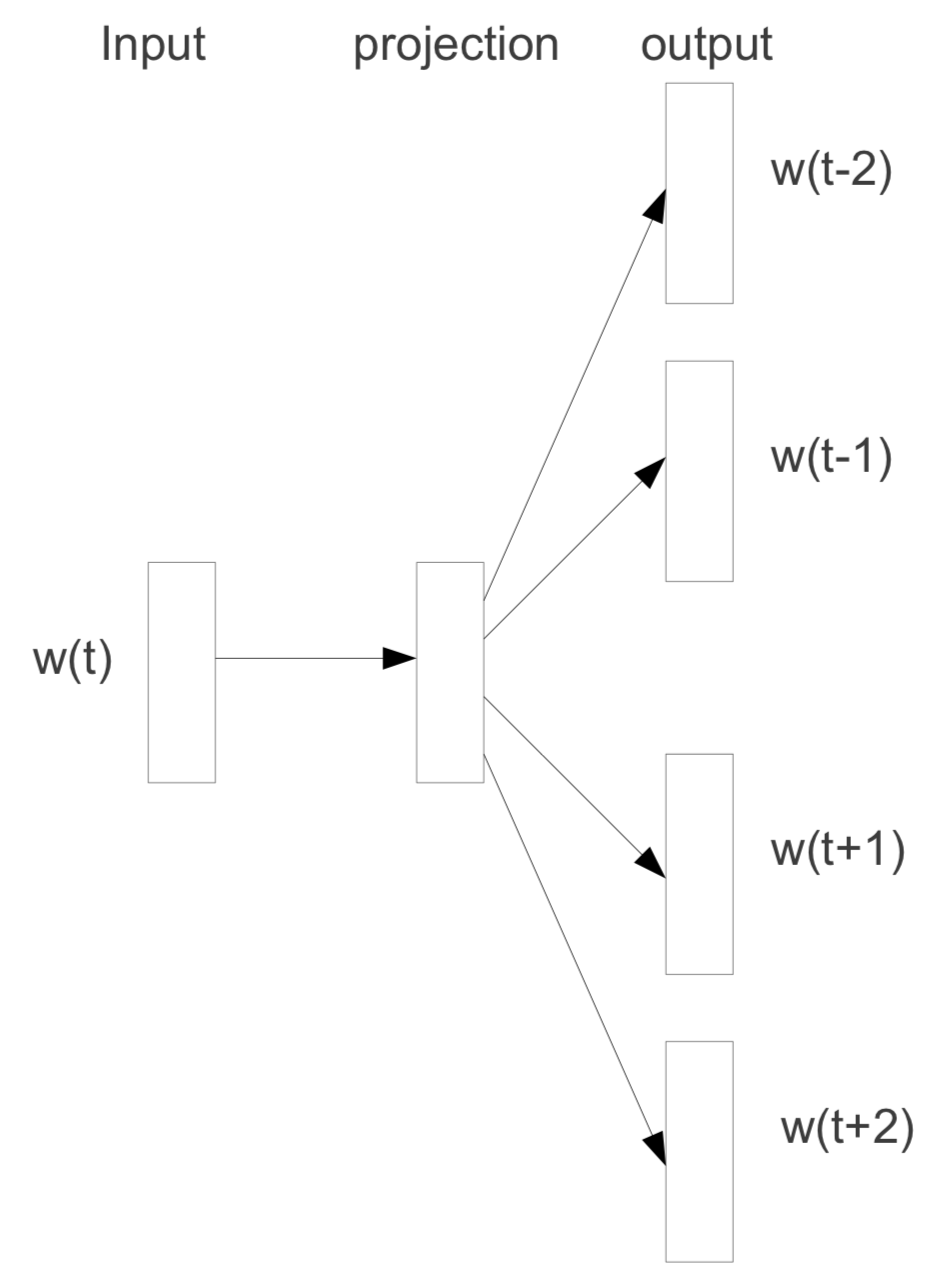
\includegraphics[width=0.35\textwidth]{figures/skip_gram.png}
\label{skip_gram}
\caption[Skip-gram]{Skip-gram model. Reprinted from \cite{mikolov_distributed_2013}.}
\end{figure}

Though being very useful, both LSA and word2vec have the same limit: they do not take into account the context when encoding a word.
In graph-based methods for solving MHQA problem, the initial node embeddings should encode not only the mentions themselves but also their context. The graph structure captures the global information in the supporting documents and their corresponding query, but throws away all the text information. Hence, I would like to enhance the graph with the local context information contained in text. In order to do so, ELMo \cite{peters_deep_2018} was deployed at the graph
construction procedural. The model consists of character-level convolution and trained 2 BiLSTM layers to encode sentences on the fly. Therefore it solves the Out-of-Vocabulary (OOV) problem naturally and enables the network to utilise morphological clues.
The word vectors from the network carry the context information passed by LSTMs forwardly and backwardly.

\subsection{Graph Neural Network}
Graph neural networks are NNs designed to process graph-structured data, or also called non-Euclidean data. Traditional NNs like fully-connected layer, CNN, and Recurrent Neural Network could not handle this kind of data, as each point in the dataset has different shape. Every graphs have different number of nodes, and each node has varying number of neighbours.

  First proposed in 2008 \cite{scarselli_graph_2009}, GNN was constructed to learn an embedding $h_v$ for each node. The embedding should contain the information of its neighbourhood. To be able to do that, we have to learn a local mapping function that is sharing among all nodes for each kind of relationship (edge), and update the embedding given its neighbour. Let $f$ be the local mapping function and $g$ be the output function, the propagation step of GNN can be defined as:
\begin{align*}
h_v &= f(x_v, x_{co[v]},\bar{h}_{ne[v]}, \bar{x}_{ne[v]})\\
o_v &= g(h_v, x_v)
\end{align*}
where $x_v$ is the feature of node $v$, $x_{co[v]}$ is the feature of its edges; $\bar{h}_{ne[v]}$ and $\bar{x}_{ne[v]}$ are the embeddings and features of $v$'s neighbour respectively. The output can be anything we care about, like node labels for node classification problem.

Although it GNN was shown to be powerful in modelling relational data, it still has some limitations:
\begin{enumerate}
\item The iterative process for updating the embeddings to reach a fixed point is not efficient. Rather we can relax the limitation and design an architecture that multiple layers of updates.
\item The parameters of the mapping functions are shared between each iteration. Instead we can make each layer of propagation having its own parameters.
\item If the node embeddings do reach a fixed point, most of the embeddings would be quite similar and it is hard to distinguish them. We would like each node's embedding contains the information of the neighbourhood, but still remains unique.
\end{enumerate}

In order to tackle these limitations and incorporate features that are suitable for modelling some particular kinds of data, researcher have proposed many variants of GNN including but not limited to Graph Convolutional Network (GCN), Graph Attention Network, Gated Graph Neural Network, GraphSAGE, ChebNet, and etc. The original GNN and its variants have achieved state-of-the-art performances in many areas including text classification, social relationship understanding, protein interface prediction, and knowledge base completion, just to name a few.


\subsubsection{GCN}
Graph Convolutional Network \cite{kipf_semi-supervised_2016} is a successfully adaptation of CNN into graph-structured data. In recent years, CNN has dominated almost all state-of-the-art leader boards and challenges in Computer Vision (CV). There are also some successful applications of CNN in NLP and speech. However, CNN is not suitable for processing non-Euclidean data, as the receptive field is hard to define due to the various number of neighbours each node has, i.e. CNN can not keep translation invariance which makes it so success in CV.,

Variants of GNN that use convolution to aggregate information can be categorised into two groups: spectral methods and non-spectral methods. The spectral methods
work with a spectral representation of the graphs: the graph Laplacian. The most simple Laplacian, combinatorial Laplacian, is defined as $L = D - A$, where $D$ is the degree matrix and $A$ is the adjacency matrix. However, most of the GCN papers utilise the concept of (symmetric) normalised Laplacian $\tilde{L} = D^{-\frac{1}{2}}LD^{-\frac{1}{2}}=I-D^{-\frac{1}{2}}AD^{-\frac{1}{2}}$ which extends Laplacian to irregular graphs. Once we get the normalised Laplacian, we can perform eigendecomposition on it: $\tilde{L}=U\Lambda U^\top$. The graph convolution operation is then defined in the Fourier domain, i.e. spectral domain, as
\[g_\theta \star x = Ug_\theta(\Lambda)U^\top x,\]
where $g_\theta$ is the filter parameterised by $\theta \in R^N$ with $diag(\theta)$, and $x \in R^N$ is the signal. Hence $U^\top x$ is just the graph Fourier transform of $x$. However, this operation is quite computationally intensive and the filter is not spatially localised.

In order to circumvent the problem, Defferrard et al. \cite{defferrard_convolutional_2016} proposed ChebNet where they approximated the filter with Chebyshev polynomials $T_k(x)$ up to order $K$:
\[g_\theta(\Lambda) \approx \sum_{k=0}^K \theta_k T_k(\tilde{\Lambda}),\]
where $\tilde{\Lambda} = \frac{2}{\lambda_{max}}\Lambda-I$ and $\lambda_{max}$ is the largest eigenvalue of $L$. The rescaled matrix $\tilde{\Lambda}$ has eigenvalues lie in $[-1, 1]$.
This way the introduced K-localised convolution removes the need to compute eigenvectors the Laplacian. Therefore we are able to stack multiple convolutional layers together to form a neural network.

Furthermore, Kipf and Welling \cite{kipf_semi-supervised_2016} limits the layer-wise convolutional operation to $K=1$ and approximates $\lambda_{max}$ with $2$ and get:
\[g_\theta \star x \approx \theta_0x + \theta_1(L-I)x = \theta_0x-\theta_1 D^{-\frac{1}{2}}AD^{-\frac{1}{2}}x,\]
which eases the overfitting on local structures on graphs that have a wide range of node degrees. Finally we get the layer-wise propagation rule in vector form:
\[H^{l+1} = \sigma(\tilde{D}^{-\frac{1}{2}}\tilde{A}\tilde{D}^{-\frac{1}{2}}H^l W^l),\]
where $\tilde{A}=A+I$ an adjacency matrix added with self-loops, $[\tilde{D}]_{ii}=\sum_j[\tilde{A}]_{ij}$ the degree matrix of the graph added with self-loops, $H^l$ is the embedding at layer $l$, $W^l$ is the layer parameter, and $\sigma$ is the non-linearity.

Though shown to have a lot potential, spectral methods is limited by that their learning process required the whole graph structure via graph Laplacian, i.e. they only work on graphs that share the same Laplacian eigenbasis, and hence can not do inductive inference on general graphs.

GraphSAGE \cite{hamilton_inductive_2017} is a general inductive framework which generates the embeddings by sampling and aggregating information from a node's neighbourhood:
\begin{align*}
h^k_{\mathcal{N}(v)} &= AGGREGATE_k(\{h^{k-1}_u|\forall u\in\mathcal{N}(v)\}),\\
h^k_v &= \sigma(W^k\cdot [h^{k-1}_v||h^k_{\mathcal{N}(v)}]),
\end{align*}
where $h_u^k$ is the embedding of node $u$ at layer $k$, $\mathcal{N}(v)$ is the set of neighbours of node $v$, $W^k$ is the parameter of layer $k$, $[\cdot||\cdot]$ is concatenation, and $\sigma$ is the non-linearity. Note that $\{h^{k-1}_u|\forall u\in\mathcal{N}(v)\}$ is not the full-set neighbour but a fixed-size uniform sample. The sampling ensures that all instances in a batch are of the same size, and modifying the sample size accordingly can alleviate the computational and memory burden. The last thing that is worth attention is the $AGGREGATE_k$, a differential aggregator function, which can be mean function, max-pooling after a fully-connected layer, or even an LSTM aggregator. When using the sum aggregator, GraphSAGE is actually an inductive variant of GCN.

\subsubsection{Relational-GCN}

All the GNNs mentioned above only deal with graphs that have single relationship, i.e. single type of edge. However, there are many graph data involving multiple relationships. For instance, Figure \ref{kg} shows part of a knowledge graph involving 4 types of edges: `played', `characterIn', `starredIn', and `genre'. Intuitively the way how information is propagated through each kind of relationship should differ, but all the models mentioned in the previous section treat all the edges as the same and fail to distinguish them.
\begin{figure}[H]
\centering
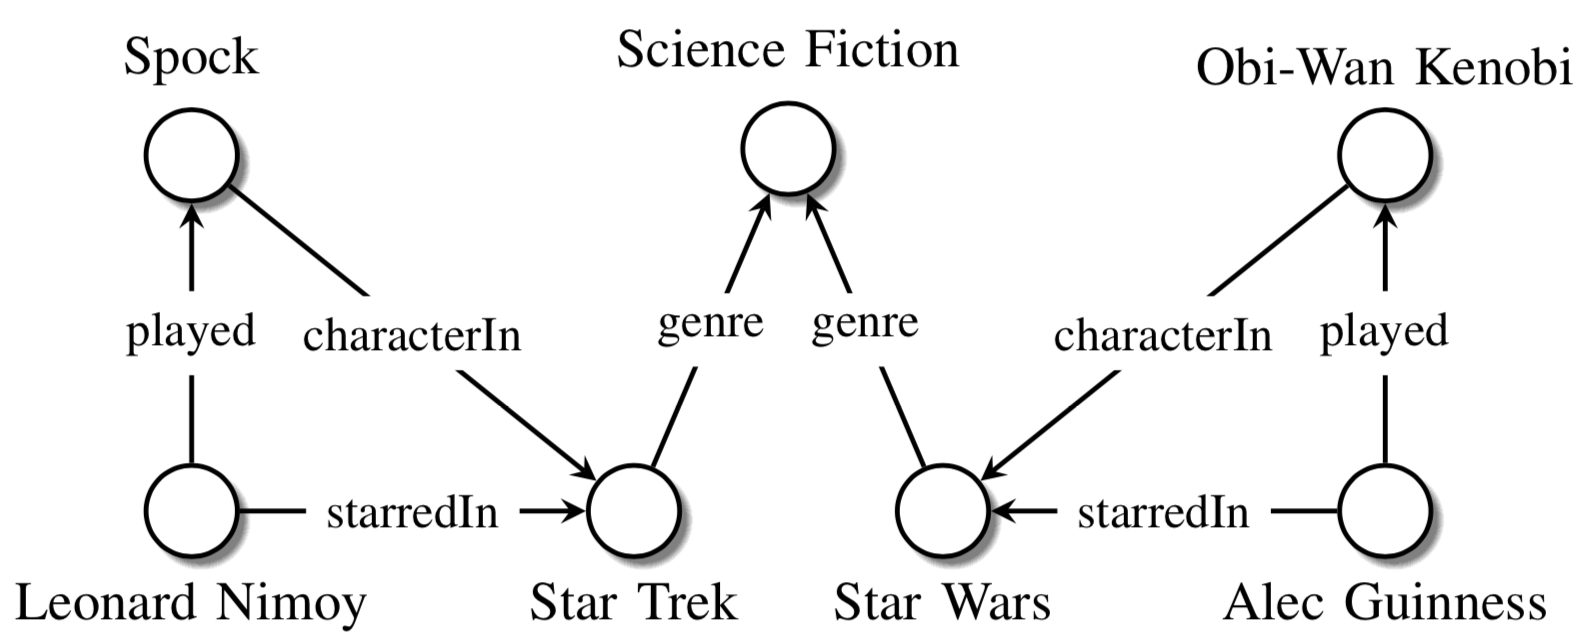
\includegraphics[width=0.9\textwidth]{figures/kg.png}
\label{kg}
\caption[Knowledge Graph]{Knowledge Graph. Reprinted from \cite{nickel_review_2016}.}
\end{figure}
Schlichtkrull et al. \cite{schlichtkrull_modeling_2018} have extended the inductive version of
GCN onto multi-relational graphs. Let $\mathcal{R}$ be the set of relationships occur in a graph, the model's propagation rule is simply:
\[h_i^{l+1} = \sigma\bigg(\sum_{r\in\mathcal{R}}\sum_{j\in\mathcal{N}_i^r} \frac{1}{c_{i,r}}W_r^l h_j^l +W_o^l h_i^l \bigg),\]
where $\mathcal{N}_i^r$ is the set of nodes linked to $i$ with relationship $r$, $c_{i,r}$ is the problem-specific normalising constant, $W_r^l$ and $W_o^l$ are the parameters, $h_j^l$ and $h_i^l$ are the embeddings of nodes $j$ and $i$ at layer $l$, and $\sigma$ is the non-linearity. Therefore the model learns to propagation information differently along different relations.

However, as we can see from the update rule, there are  $|\mathcal{R}|$ times more parameters in Relational-GCN (R-GCN) comparing to GCN, which significantly increases the risk of over-parameterisation. To mitigate the risk, regularisations including
basis decomposition and block-diagonal decomposition are introduced. With the basis decomposition, each weight $W_r^l$ is defined as:
\[W_r^l = \sum_{b=1}^B a_{rb}^l V_b^l,\]
where $B \leq |\mathcal{R}|$ is the number of basis, $V_b^l \in \mathbb{R}^{d^{l+1}\times d^l}$ is the $b$-th basis, and $a_{rb}^l$ controls how the base are combined to form the parameters for relationship $r$. In block-diagonal decomposition, we have
\[W_r^l = \bigoplus^{B}_{b=1}Q_{br}^l,\]
a direct sum over a set of lower-dimensional matrices $\{Q_{br}^l \in \mathbb{R}^{(d^{l+1}/B)\times(d^l/B)}\}$.

\subsection {Link Prediction}
Given an arbitrary graph, Link Prediction (LP) tries to find out whether there are links between two ore more entities. As graphs are omnipresent in real world, LP has a wide range of applications including friend recommendation \cite{adamic_friends_2003}, product recommendation \cite{talasu_link_2017}, knowledge base completion \cite{nickel_review_2016}, and crime prevention \cite{berlusconi_link_2016} by predicting missing links in the crime network. In the early days researchers have developed a bunch of straightforward yet competent heuristics for evaluating the similarity of nodes such as common neighbours, preferential attachment \cite{barabasi_emergence_1999}, Adamic-Adar \cite{adamic_friends_2003}, resource allocation \cite{zhou_predicting_2009}, and SimRank \cite{jeh_simrank:_2002}.
Based on how similar two nodes are, we can then set or train a threshold to determine if there is link between them.

All the methods mentioned above utilizes the local or global graph structures, but do not take into account the differences between nodes and the type of the edges. In order to encode useful information other than the graph structures, people have proposed methods incorporating graph embedding. This kind of methods  can work on graphs with node embedding initialised with information retrieval or NLP methods like word vectors \cite{mikolov_distributed_2013}. With word embedding, the contextual information is projected into a lower dimensional space at where the distance/relationship between two nodes can be easily resolved. Below some of these methods are introduced and compared.

\subsubsection{TransE}
Bordes et al. \cite{bordes_translating_2013} proposed to model entities and relationships in the same embedding space $\mathbb{R}^d$. Therefore all the vectors can operate with each other directly, and the relationship is just a vector that linearly interacts with
the vectors of entities.
Given a triplet $(s, r, t)$ from the knowledge base representing nodes $s$ and $t$ are related by edge $r$, we want to have $\mathbf{s}+\mathbf{r}\approx\mathbf{t}$, i.e. $\mathbf{t}$ is the nearest neighbour of $\mathbf{s}+\mathbf{r}$. Otherwise if the triplet is from negative sampling we want them to be far apart. Note that all the entity vectors are unit vectors to narrow the embedding space. To learn such embeddings a margin-based ranking loss is minimized over the train set:
\[\mathcal{L} = \sum_{(s,r,t)\in S}\sum_{(s^\prime,r,t^\prime)\in S_{(s,r,t)}}[\gamma+d(\mathbf{s}+\mathbf{r}, \mathbf{t})-d(\mathbf{s^\prime}+\mathbf{r},\mathbf{t^\prime})]_+,\]
where $S$ is the knowledge base, $S_{(s,r,t)}$ is the set of negative samples of $(s,r,t)$ where the source or target is corrupted, $\gamma$ is the margin we want between the positive and negative samples, $d(a, b)$ is the metric like Manhattan or Euclidian distances defined in $\mathbb{R}^d$, and $[x]_+=max(0,x)$.

There are two extensions of TransE: TransH \cite{wang_knowledge_2014} learns different entity embeddings for different kind of relationship, hence the goal is simply to make $\mathbf{s}_r+\mathbf{r}$ and $\mathbf{t}_r$ close to each other for positive samples and far away otherwise; TransR \cite{lin_learning_2015} learns a project operator $M_r$ for relation $r$ to project $\mathbf{s}$ and $\mathbf{t}$ onto $\mathbf{s}_r$ and $\mathbf{t}_r$, hence it does not need to keep $N\times|\mathcal{R}|$ distinct embeddings but just $N$ embeddings and $|\mathcal{R}|$ operators.

However, the relations considered in these approaches are all linear operators represented by one-dimensional vectors which is very limiting. The model lacks the ability to model the interaction between entities. Hence some other researchers have proposed to model the relations bilinearly.

\subsubsection{NTN}
Socher et al. \cite{socher_reasoning_2013} proposed to use Neural Tensor Network (NTN) to do knowledge base completion. In NTN, one node's embedding is initialised by applying mean pooling to the word vectors corresponding to the entity of that node and so, not like in TransE, the embedding is not a unit vector like anymore.
The scoring function, a bilinear tensor layer, is defined as:
\[g(s, r, t)=u_r^\top\sigma\bigg(s^\top W_r^{[1:k]}t+V_r\begin{bmatrix}s \\
t \\
\end{bmatrix}+b_{r} \bigg), \]
where $\sigma$ is the non-linearity which was $tanh$ chosen by the authors, $W_r^{[1:k]}\in\mathbb{R}^{d\times d\times k}$ is a tensor such that $s^\top W_r^{[1:k]}t$ results in a vector in $R^k$, $V_r\in \mathbb{R}^{k\times 2d}$, and $u_r, b_r \in \mathbb{R}^k$. The objective is to train the scoring function so that it returns $1$ for positive samples and $-1$ otherwise. This way the model is capable of modelling the interaction between entity vectors and the linear matrix operator and non-linearity further enhance the model's expressiveness. Nonetheless the model now suffers from the risk of over-parameterisation and higher computational burden.

\subsubsection{DistMULT}
DistMULT \cite{yang_embedding_2014} was proposed by Yang et al. to simply the scoring function of NTN yet achieve similar or even better performance in link prediction. The non-linearity and linear matrix in NTN are removed, and the bilinear tensor is replaced by a bilinear matrix such that the scoring function is now:
\[g(s,r,t) = \mathbf{s}^\top W_r\mathbf{t},\]
where $(s,r,t)$ is the triplet representing source node $s$, relation (edge) $r$, and target node $t$. Similar to NTN the scoring function is trained to produce $1$ for positive samples and $0$ for negative samples. To facilitate training, the margin-based ranking loss which was used by TransE is incorporated into the model. Also note that the entity representations $\mathbf{s}$ and $\mathbf{t}$ can be n-hot vectors or vectors produced by word embedding techniques which capture local context to aid the inference on global graph structure. Nevertheless, people have found that DistMULT works pretty well on standard graph data, but is not good at modelling asymmetric relations. To deal with that people have introduced complex number into the embeddings and parameters, which shows prominent improvements over DistMULT on graph-structured data with asymmetric relations.

\subsubsection{R-GCN}
As detailed above, R-GCN is a GNN model that propagate information in multi-relational graphs. The ability to accumulate evidence through several inference steps on the graph can further improve the factorisation models for link prediction like DistMULT, NTN, and TransE described before. Schlichtkrull et al. chained an R-GCN as the encoder with a scoring function as the decoder to get a graph auto-encoder \cite{kipf_variational_2016} as shown in Figure \ref{lp_model}. Evaluation on WN18, FB15K, and FB15K-237 \cite{toutanova_observed_2015} datasets have shown improvements over other link prediction models without the encoder.
\begin{figure}[H]
\centering
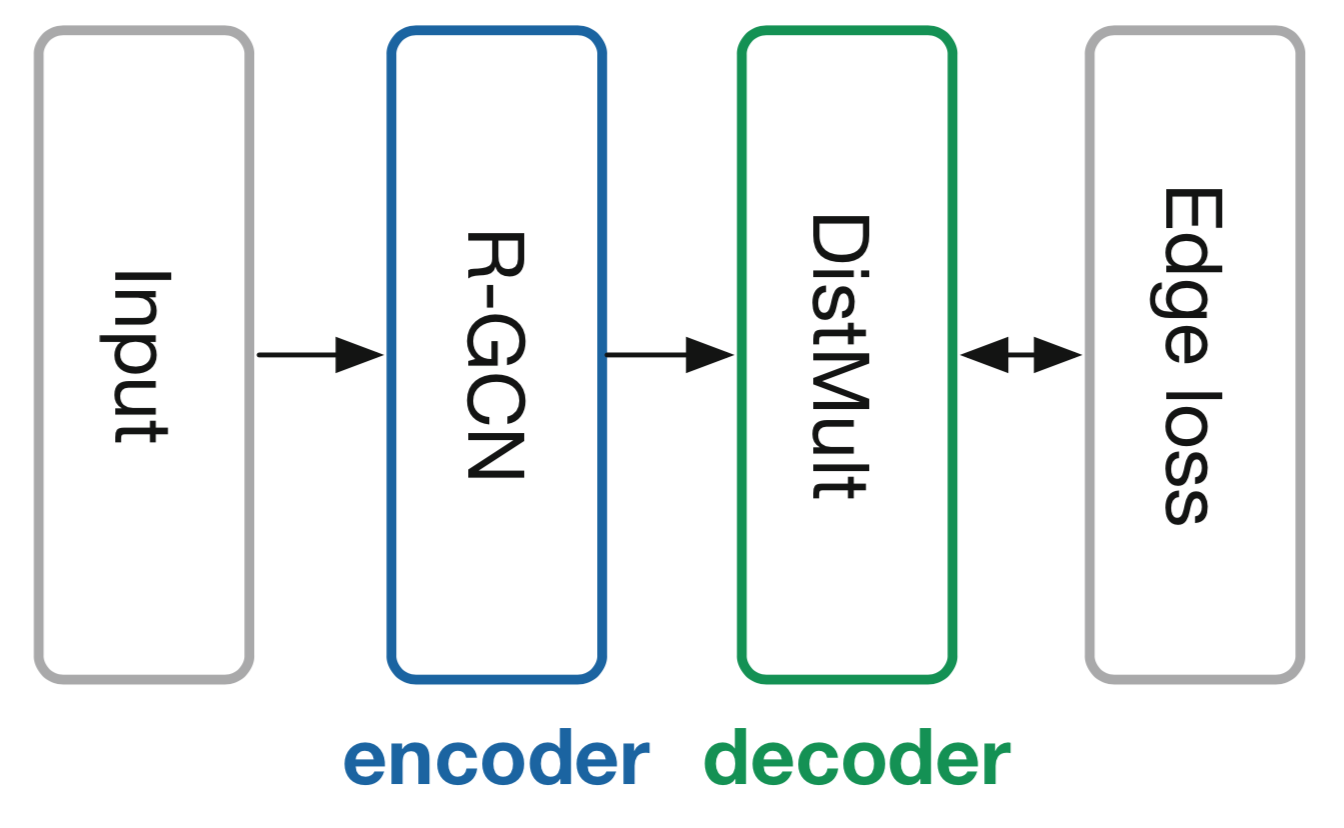
\includegraphics[width=0.4\textwidth]{lp_model.png}
\label{lp_model}
\caption[The Link Prediction Model with R-GCN]{The Link Prediction Model with R-GCN. Reprinted from \cite{schlichtkrull_modeling_2018}.}
\end{figure}

\subsubsection{ConvE}
Dettmers et al. \cite{dettmers_convolutional_2017} hypothesised that with a much deeper model the learned feature may be more expressive than those learned with shallower models. Hence they proposed to use a multi-layer 2D convolutional neural network
to perform link prediction tasks. The scoring function of their model is:
\[g(s,r,t) = \sigma(vec(\sigma([\bar{\mathbf{s}}||\bar{\mathbf{r}}]*\omega))W)\mathbf{t},\]
where $\sigma$ is the non-linearity which was ReLU in the paper, $\mathbf{s}, \mathbf{t}$, and $\mathbf{t} \in \mathbb{R}^d$ are the entity vectors and relation vector respectively, $\bar{\mathbf{s}}, \bar{\mathbf{r}} \in \mathbb{R}^{d_w\times d_h}$ where $d_w\times d_h = d$ are the 2D reshaped $\mathbf{s}$ and $\mathbf{r}$, $\omega$ is a convolutional filter, and $W$ is the layer projection parameter. Unlike all factorisation models mentioned above which used margin-based ranking loss, a BCE loss is minimised over all edges (positive and negative) to train the model. As convolutional operation is far more parameter efficient than linear and bilinear operations, the ConvE model produces similar performance to DistMULT and R-GCN with 8 times and 17 times fewer parameters, i.e. it significantly soothes the risk of over-parameterisation. 
% Figure \ref{conve} shows the whole running procedure of ConvE.
% \begin{figure}[H]
% \centering
% 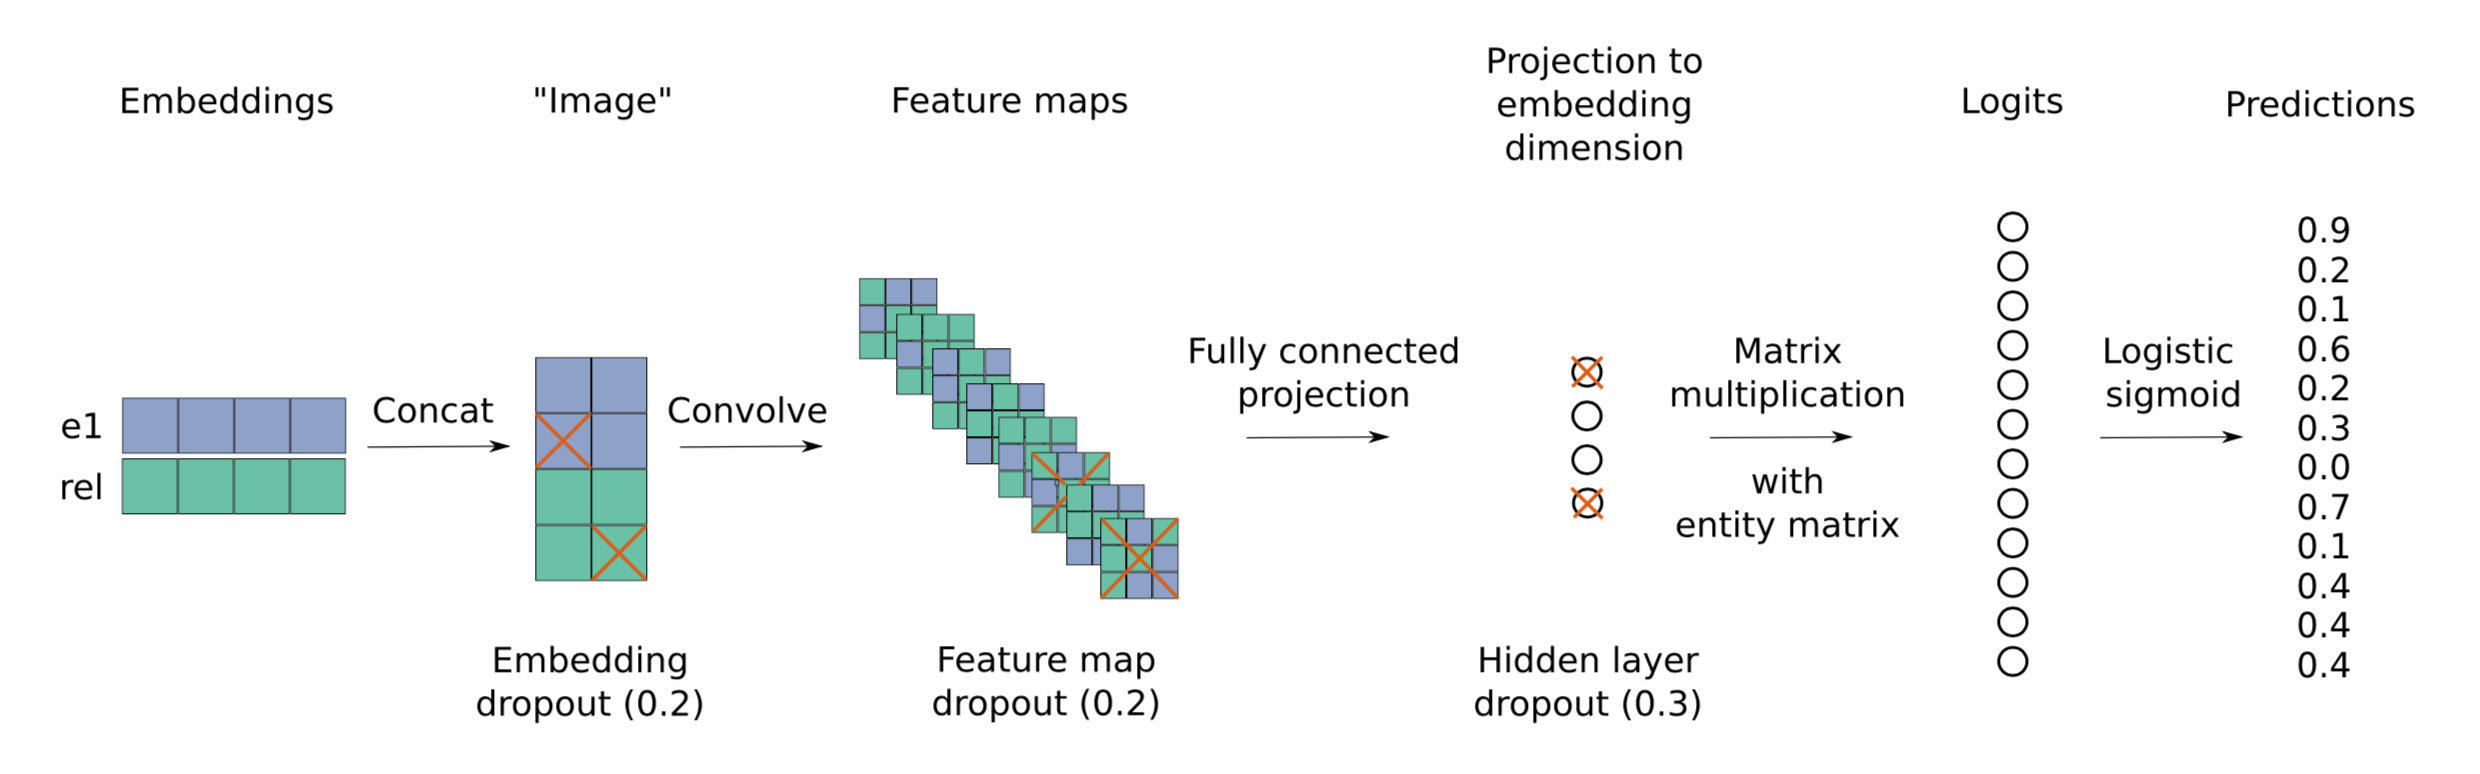
\includegraphics[width=1.\textwidth]{figures/conve.png}
% \label{conve}
% \caption{ConvE model. Reprinted from \cite{dettmers_convolutional_2017}.}
% \end{figure}


\section{Related Work}
\subsection{MHQA on Knowledge Bases and Sentences}
Many existing works on multi-hop reasoning focused on hopping over knowledge bases \cite{jain_question_2016, neelakantan_neural_2015, yin_neural_2016} which do not require the system to be able to comprehend text but only known relations with well-defined structure. In order to inspire the creation of such a system that can perform multi-hop QA on textual data, many datasets which require the model to reason across multiple sentences including bAbI \cite{weston_towards_2015}, OpenBookQA \cite{mihaylov_can_2018}, CBT \cite{hill_goldilocks_2015}, and MultiRC \cite{shen_reasonet:_2017} were introduced. Many systems \cite{sun_improving_2019, wu_global--local_2019} have been proposed to solve these multi-hop reading comprehension tasks. However, the problem we are interested in is to aggregate information from multiple documents, since the most popular data interspersed in the real world are unprocessed, textual documents but not sentences or knowledge bases.

One line of approaches that deal with multiple passages try to select the most relevant document first before performing reading comprehension to answer the question \cite{chen_reading_2017, dhingra_quasar:_2017, clark_simple_2018,wang_r$^3$:_2017,dunn_searchqa:_2017}. Nonetheless this kind of methods fail to accumulate information across documents, but reduce the problem into two easier problems: a classification problem to choose the most relevant document, and then a reading comprehension problem to answer the question. 

To address the problem of combining information from different documents before making the decision, a few approaches \cite{wang_evidence_2017, wang_joint_2018, lin_denoising_2018} have been proposed to aggregate the contexts of   the same candidate in different passages to cover various aspect of the question. However, these approaches fail in combining evidences from the contexts of different entities which could be of concern for answering the question properly. 

\subsection{MHQA with Attention-Based Methods}
Neural attention mechanism \cite{bahdanau_neural_2014} trains a selector network to weight and combine the outputs from the last layer/encoder accordingly to form the input for the next layer/decoder. This design resembles the biological attention mechanism where our brains selectively concentrate on a distinct aspect of information while neglecting other perceivable information. With the help of attention, researchers have design many approaches that properly accumulate information from multiple passages according to the query. Furthermore, multi-hop attention mechanism helps to focus on different aspects on different step to simulate the reasoning chain for answering the question.

BiDAF \cite{seo_bidirectional_2016} and FastQA \cite{weissenborn_making_2017} were introduced into the MHQA problem by Welbl et al. \cite{welbl_constructing_2018}. Although originally designed for processing single document, these two methods were adapted successfully to work on a super-passage constructed by concatenating all documents randomly. MHPGM \cite{bauer_commonsense_2018} proposed by Bauer et al. uses multi-attention mechanism to perform multi-hop reasoning and a pointer-generator network to synthesise the answer.  Moreover external commonsense information is extracted from ConceptNet \cite{speer_conceptnet_2016} to fill in the gaps of reasoning between hops using a gated attention mechanism. Weaver \cite{raison_weaver:_2018} performs co-encoding through several BiLSTM layers to relate the question to the documents, then use a memory network \cite{sukhbaatar_end--end_2015} to make the question attend to the context iteratively before making the decision.

More recently, Zhong et al. proposed CFC \cite{zhong_coarse-grain_2019} which uses co-attention and self-attention to encode the documents with respect to the question and then score each candidate by comparing its occurrences throughout all documents with the question. DynSAN \cite{zhuang_token-level_2019} approaches the problem from token-level by choosing the important tokens with a gated token selection mechanism first, then use self-attention mechanism to model their dependencies with the help of convolutional layers.

The last work to be present is the Coref-GRU proposed by Dhingra et al. \cite{dhingra_neural_2018}. Although the method itself is not graph-based, it inspires the line of research on MHQA using GNN models. This method encodes the relation between mentions of entities with coreference, then an GRU augmented with jump links is used to aggregate the information across documents.
\subsection{MHQA with Graph-Based Methods}
This work follows the idea of graph-based MHQA methods and tries to improve them by augmenting the graph extracted from the documents with link prediction. The first attempt to use GNN for multi-hop reasoning was MHQA-GRN proposed by Song et al. \cite{song_exploring_2018}. This model consists of a BiLSTM (or Coref-BiLSTM which is the LSTM adaptation of Coref-GRU)
to encode the local context of each entity mention, a few GNN
layers to propagate information through the graph structure to perform the reasoning, and
a fully-connected network to predict the answer. It outperformed all other models that do not utilise graph structure at the time it was published. However, this method does not take into account the query information when encoding the entity mentions, and does not distinguish the types of edges which may be essential for reasoning over the relationships among the entities. Entity-GCN proposed by De Cao et al. \cite{de_cao_question_2019} address the problems mentioned above. After encoding the query and entity mention with LSTM, query embedding is concatenate with each entity embedding and then pass through a feed forward fully-connected network to combine the query information into the entity information. Also, all relationships are now treated differently with the help of R-GCN to propagate information differently along various types of edges.

HDEGraph proposed by Tu et al. \cite{tu_multi-hop_2019} further improves the result by extending the graph which has all of its nodes being entity mentions into a heterogeneous graph: a graph consists of document nodes, candidate nodes, and entity nodes. Moreover, the number of types of edges is increased to seven from four. Finally, the co-attention and self-attention mechanisms for encoding the documents are adapted from CFC to get a better initialisation of node embeddings. BAG proposed by Cao et al. \cite{cao_bag:_2019} tries to incorporate attention mechanism into graph by deferring the integration of query information into entity information until the R-GCN layers have accumulated the relational information
over the entity graph to form relation-aware node embeddings. Then a bidirectional attention layer (node2query and query2node) is applied to produce the query-relation-aware node embeddings which are then passed into a fully-connected network to predict the answer. Note that the initial node features are a combination of ELMo and GloVe \cite{pennington_glove:_2014} embeddings.

\chapter{Methodology}
This chapter consists of detailed descriptions of the design of the two models: one without link predictor and one that has. The two models are compared to investigate the effect of performing link prediction for MHQA tasks. Then the plan for implementation and testing of the models are articulated, with a discussion of the contribution of this dissertation follows.

\section{Model Design}
There are two models of consideration: one of them comprises only the entity graph extracted from the documents and a few R-GCN layers for propagating information, the other one consists of an additional link predictor to complete the entity graph before passing the graph into the R-GCN layers.

\subsection{Model Without Link Predictor}
The model without link predictor is very similar to that of Entity-GCN with a few modifications. It is built for providing a baseline for the one with facilitation of link prediction. This model consists of four parts: an encoder for summarising the local contexts of entity mentions, the entity graph extracted from the documents, an R-GCN network that propagates information on the entity graph,
and a fully-connected network to predict the answer.\subsubsection{Encoder}
As we discussed earlier, pre-trained word embedding techniques have boosted the performance of many downstream NLP tasks. The gargantuan corpus the embeddings are trained on and the tremendously many steps they are trained for help them to capture the statistical relationships between words and context. Since we have neither a large training corpus nor the necessary computational resources, an contextualised embedding, ELMo, but not a self-trained word encoder is used to obtain the initial word embeddings for entity mentions.
Also, the lightweight encoding part achieved by using the pre-trained embedding makes the system to be able to run in real-time.

For an entity mention $[w_1,\dots,w_n]$ of $n$ words, we first get the pre-trained contextualised ELMo embeddings $[{\mathbf{w_1},\dots,\mathbf{w_n}\in\mathbb{R}^{3072}}]$. However, what we want is a single vector embedding for each entity mention. Unlike what was done in Entity-GCN where the first and last word vectors are concatenated to form $[\mathbf{w_1}||\mathbf{w_n}]\in\mathbb{R}^{6144}$ as the entity encoding, I take the element-wise mean of all word vectors to get $x^{\prime}=(\mathbf{w_1}\oplus\cdots\oplus\mathbf{w_n})\oslash n\in\mathbb{R}^{3072}$ as the initial entity encoding to reduce the number of parameters needed for the following encoding steps. Then $x^\prime$ is passed into a linear layer and a ReLU activation to get $x\in\mathbb{R}^{256}$.

For the query of $n$ words we also get the ELMo embeddings $[{\mathbf{w_1},\dots,\mathbf{w_n}\in\mathbb{R}^{3072}}]$ first. Then we do not perform the mean pooling, instead the sequence is passed into two BiLSTM layers of which the hidden dimensions are 256 and 128 respectively. The last two outputs from the later BiLSTM layer, $\overrightarrow{q_n}\in\mathbb{R}^{128}$ and $\overleftarrow{q_n}\in\mathbb{R}^{128}$, are then concatenated to form the query encoding $q:=[\overrightarrow{q_n}||\overleftarrow{q_n}]\in\mathbb{R}^{256}$.

This way we have the query encoding $q$ and entities encodings $\{x_1,\dots,x_N\}$ which summaries their local contexts. Furthermore, we would like the entity encodings to be query-aware so that the R-GCN layers propagates information with the query taken into concern. Hence we concatenate the query embedding with each entity encoding vector to get $\{[x_1||q],\dots,[x_N||q]\in\mathbb{R}^{512}\}$ which are then passed into two layers of fully-connected network of which the hidden dimensions are 1024 and 512 respectively to get the query-aware entities encodings $\{\hat{x_1},\dots,\hat{x_N}\in\mathbb{R}^{512}\}$.

\subsubsection{Entity Graph}
The content of each training instance, i.e. the query and its supporting documents, is organised into a graph. The nodes are mentions of entities, the candidates and query entity, in all documents, note $\{v_1,\dots,v_N\}$. All the queries are prepared in the form of $q=<s,r,?>$ where $s$ is the subject, $r$ is the relation, and $?$ is the object which should be chosen among the candidates. Hence it is easy to separate the subject $s$ in the query to be used as the query entity.

Apart from exact matching of entities, coreference resolution system \cite{wiseman_learning_2016} is used to extend the set of nodes in the graph. Specifically, for each coreference chain, if any of the entities are included in the chain, all other named entities in that chain will be added as new nodes. However, if any mention is resolved ambiguously into more than one coreference chains, it is discarded from the set of nodes to avoid the R-GCN network propagates vagueness.

All the nodes collected as described above in this subsection is then encoded as detailed in the last subsection to get the initial node embeddings $\{h_1^0, \dots,h_N^0\in\mathbb{R}^{512}\}=\{\hat{x_1},\dots,\hat{x_N}\in\mathbb{R}^{512}\}$. The edges defined below are then constructed to connect these mentions together:
\begin{enumerate}
\item SAME-DOC edges: if they appear in the same document;
\item MATCH edges: if they are exact match;
\item COREF edges: if they occur within the same coreference chain;
\item COMPLEMENT edges: if they are not connected to any other nodes by the three kind of edges mentioned above, i.e. they are isolated.
\end{enumerate}

\subsubsection{R-GCN Network}
Since there are four types of edges, R-GCN is a natural choice for propagating information over this multi-relational graph. The reasoning chain is assumed to be captured by propagating local information along the edges, hence to simulate the reasoning chain properly we need a multi-hop propagation which leads to a multi-layer R-GCN networks. As suggested by the original paper $L=3$ layers are used, since increasing the number of layers does not improve the performance anymore but cause the vanishing gradient problem.

Instead of using the vanilla R-GCN layer, a gated version of it is deployed so that the network learns to control how much information is propagated to the next step. If a reasoning chain has length less than three, the gating mechanism should be able to stop the model from propagating information further away and blur the correct answer.

Recall that R-GCN layer updates node representations by:
\[u_i^{l+1} = \sigma\bigg(\sum_{r\in\mathcal{R}}\sum_{j\in\mathcal{N}_i^r} \frac{1}{c_{i,r}}W_r^l h_j^l
+W_o^l h_i^l \bigg).\]
Instead of setting $h_i^{l+1}=u_i^{l+1}$ directly, we train a linear layer $f_a$ with sigmoid activation:
\[a_i^{l+1}=\sigma(f_a([u_i^{l+1}||h_i^l]))\]
to form the update gate and apply the update accordingly:
\[h_i^{l+1}=\phi(u_i^{l+1})\odot a_i^{l+1}+h_i^l\odot(1-a_i^{l+1}),\]
where $\phi$ is a $tanh$ layer chosen as the non-linearity. Note that to reduce the number of parameters, all 3 R-GCN layers share the same parameters and hence the introduction of the gating mechanism is necessary for distinguishing each layer. 

\subsubsection{Output Network}
After the graph is passed through the 3 R-GCN layers, we get the final node representations $\{h_1^3, \dots,h_N^3\in\mathbb{R}^{512}\}$. The Entity-GCN then computes the probability of choosing a candidate $c$ as the answer by:
\[p(c|q) \propto exp\bigg(\underset{i\in\mathcal{M}_c}{max} f_o([q||h_i^3])\bigg),\]
where $\mathcal{M}_c$ is the set of indices such that node $i$ is a mention of candidate $c$ and $f_o$ is the fully-connected output network. Instead we remove the $max$ operation and treat each node individually by computing:
\[p(i|q)=\sigma(f_o([q||h_i^3])),\]
where $\sigma$ is the sigmoid activation, i.e. $p(i|q)$ is the probability whether the mention corresponding to node $i$ is the correct answer. This way we transformed the CE loss as a BCE loss and the multi-class classification problem is reduced as $N$ binary classification problems. The output network $f_o$ is a three layers fully-connected model with hidden dimensions 256, 128, 1 for each layer.

\subsection{Model with Link Predictor}
The only difference between this model with link predictor and the baseline model is that there is a link predictor, namely R-GCN link predictor, between graph construction and the message propagation network. Therefore, the description of encoder, entity graph, message propagation network, and output network is omitted in this subsection.

\subsubsection{Link Predictor}
There is a choice between R-GCN and ConvE. As ConvE is deeper than R-GCN, it can produce better learned features for complex graphs. More specifically, it outperforms R-GCN on graphs with node degrees greater than 10,000. Whereas for simpler graph R-GCN achieves better performance in link prediction than ConvE does. Hence an investigation into the entity graphs built for the QAngaroo WikiHop dataset is carried out to decide which model should be applied. The result of investigation is shown in Table \ref{graph_stat}. As we can see the entity graphs built are not very complex, and even the most complex graph has the maximum node degree
being 317 which is much smaller than 10,000.\begin{table}[H]
\center
\caption{Statistics of Entity Graphs Built}
\label{graph_stat}
\begin{tabular}{l|lllll}
     & \# nodes & \# edges & min degree & avg degree & max degree \\ \hline
Mean & 67.41    & 2745.70  & 1.57       & 15.58      & 27.70      \\
Max  & 611      & 137962   & 33         & 268.58     & 317       
\end{tabular}
\end{table}

Therefore, R-GCN is deployed to perform graph completion. The predictor consists of two R-GCN layers for encoding the graph and a DistMULT decoder for scoring the triplets sampled. Two R-GCN layers both have the output dimension being 512 which is the same as that of the initial node embeddings. For simplicity the basis decomposition
layer is used and the number of bases is the same as the number of relations, i.e. $B=|\mathcal{R}|=4$. After the graph being passed through the encoder we have the final node representations $\{h_1^2, \dots,h_N^2\in\mathbb{R}^{512}\}$ of which will then be fed into decoder for scoring the given triplets.

Like I mentioned before, the DistMULT decoder scores an edge bilinearly:
\[g(i,r,j)=\sigma\big((h_i^2)^\top W_rh_j^2\big),\]
where $W_r \in\mathbb{R}^{512\times512}$ is a diagonal matrix, 
and therefore $W_r$ can be parameterised as $diag(\{W_r^{(1)},\dots,W_r^{(512)}\})$; $\sigma$ is the sigmoid activation.

To train the predictor, negative sampling is used to construct the training instances. For each edge in the edge set $\{(s,r,t)\}$ of an entity graph built, we randomly corrupt its source or target to get the negative sample $(s,r,t^\prime)$ or $(s^\prime,r,t)$ which is not in $\{(s,r,t)\}$. For positive samples, i.e. edges/triplets in the original edge set, the labels are 1; for negative samples in the corrupted edge set $\{(s^\prime,r,t^\prime)\}$ the labels are 0.
Hence BCE loss can be applied to train the predictor. During testing phase, only edges with $g(s,r,t)>0.5$ is accepted and added into the edge set of the entity graph.

\section{Implementation}
The original R-GCN and Entity-GCN papers run their experiments on CPU due to that the large amount of memory required to run vectorised computation cannot be fulfilled by GPU. In this project we would like to build a pipeline which utilise the parallelism provided by GPU with the help of mixed precision training.

Firstly spaCy is used to perform named entity recognition which extracts the potential nodes of the entity graph. NeuralCoref built on top of spaCy is then deployed to resolve coreference which gives the coreference chains needed to decide which entities to add in the entity graph, and construct the COREF edges. Then AllenNLP \cite{gardner_allennlp:_2018} with pre-trained ELMo embedding is applied to encode the local context of mentions of entities.

 The edges constructed and the nodes being initialised by encoder are then packed into the graph Data object of PyTorch Geometric (PyG) \cite{fey_fast_2019}, a geometric deep learning framework, which is built on top of PyTorch \cite{paszke_automatic_2017} that supports tensor computation on GPU. All the models are then built with PyTorch and PyG.

The instantiated models are then wrapped by Apex \cite{micikevicius_mixed_2017} to allow automatic casting during the process of forward pass to reduce the memory used, and loss scaling in the backward pass to preserve small gradient values.

\section{Testing}
Testing is performed on the development set of QAngaroo WikiHop dataset, as the testing set is not published. The accuracies achieved by these two models (with and without link predictor) on the development set are then compared to decide whether the use of link prediction helps solving MHQA problems.

\section{Contribution}
This study investigates the effect of performing graph completion through link prediction on solving MHQA problems with graph-based methods. It also builds a pipeline that utilised mixed precision training to allow the model to be run on GPU to circumvent the limitation of memory size.


\chapter{Experimental Results}
In this chapter the set-up of the experiments like the hyperparameters used is discussed. Then the results are presented with the evaluation of them.

\section{Set-Up of Experiments}
\section{Results}
\section{Assessment}

\chapter{Conclusion}
\section{Summary}

\section{Future Work}
\subsection{Encoder ...}
BERT, XLNet, co-attention, self-attention, ...

\subsection{Deeper GNN ...}
However, the GNNs we have seen for now are very `shallow' - around three or four
layers due to vanishing gradient problem. As we know it now, the power of neural network comes from building
the network to be very deep. In order to tackle this problem, Li et al. \cite{li_deepgcns:_2019} borrowed
the idea of residual and dense connections from Convolutional Neural Networks (CNNs) and trained a GCN
that is as deep as 56 layers. As a result that network has beaten other GCNs with only few layers ...

\subsection{Link Prediction ...}
Though the graphs built do not shows too much asymmetric relations, changing the decoder of RGCN to ComplEx may still improve the performance ...

\subsection{HotpotQA ...}


\appendix
\bibliographystyle{plain}
\bibliography{ref}

%\chapter{Appendix}

\end{document}
